\documentclass[reprint,superscriptaddress,prb,showkeys]{revtex4-2}
\usepackage{empheq}
\usepackage{float}
\usepackage{lipsum}
\usepackage{mathtools, cuted}
\usepackage{esvect}
\usepackage{xcolor}
\usepackage[caption = false]{subfig}
\usepackage{graphicx}
\usepackage{dcolumn}
\usepackage{bm}
\usepackage{hyperref}
\usepackage{physics}
\usepackage[mathlines]{lineno}
\usepackage[capitalise]{cleveref}
\usepackage[english]{babel}
\usepackage{orcidlink}
\usepackage{natbib}
\usepackage{amsmath}
\usepackage{amssymb}


%------------- COMMANDS -------------

\newcommand{\C}{\mathbb{C}} %complex
\newcommand{\R}{\mathbb{R}} %reals
\newcommand{\Z}{\mathbb{Z}} %integers
\renewcommand{\P}{\mathbb{P}} %prob

\newcommand{\m}{\text{m}} %m index
\newcommand{\M}{\text{M}} %m index
\newcommand{\N}{\text{N}} %n index
\newcommand{\n}{\text{n}} %n index
\renewcommand{\a}{\textbf{\text{a}}} %a index

\newcommand{\brac}[1]{\left(#1 \right)} %nice brackets
\newcommand{\bk}[1]{\langle #1 \rangle} 

\newcommand{\TODO}[1]{\textcolor{red}{TODO: #1}}


%------------- MAIN -------------

\begin{document}

\title{Efficient Machine Learning in a Memristor Network}

\author{Monica Conte}
\affiliation{Soft Condensed Matter \& Biophysics, Debye Institute for Nanomaterials Science, Utrecht University, Princetonplein 1, 3584 CC Utrecht, The Netherlands.}

\date{\today}

\begin{abstract}
Inspired by the brain's energy-efficient processing, we propose a physical implementation of artificial neural networks to surpass digital systems in speed and energy efficiency. We consider a network with nodes connected by conical microfluidic memristor channels filled with aqueous electrolyte [1]. These memristors exhibit tunable conductance, responsive to electrical, chemical, and mechanical stimuli, as well as channel geometry. Based on this adaptability, we develop a hybrid training algorithm that adjusts either channel geometry or external stimuli as weights. Physical relaxation replaces the feedforward pass, while a combined physical-numerical gradient descent drives the backward pass. This approach enables tasks such as input-output voltage mapping and linear regression.
\end{abstract}
\maketitle

\renewcommand{\figurename}{FIG.}

\section{\label{sec:Intro}Introduction}

% ## Artificial Neural Networks ##
% - What they can achieve
% - Energy cost
% - Explain the two phases

Artificial neural networks (ANNs) have become central to many technological advancements, achieving remarkable success in tasks ranging from image recognition to natural language processing. These networks typically operate in two phases: inference and backpropagation. The energy requirements of ANNs has grown significantly, negatively impacting the efficiency and scalability of ANNs\cite{energy_cost}.

% ## Physical Neural Networks ##
% - what they are, what is the scope (physical instead of math training)
% - advantages: faster, computations are less energy demanding. 

While the inference energy consumption has been addressed by hardware accelerators, the backpropagation still remains a problem. As an alternative to ANN performed strictly in-silico, physical neural networks (PNN) have been introduced, where physical processes rather than mathematical operations are trained\cite{}. In fact, physical processes are often faster and consume less energy than their digital counterpart. 

% ## PNN algorithms in literature ##

% ## Our networks and our algorithm ##

Not only, but physical neural networks make the similarity with the human brain more evident, opening the doors to the development of an artificial brain. For this, we choose to work with networks whose constructing elements are memristors living in aqueous solution and that respond to electrical, chemical and mechanical stimuli at the same time.

Fluidic channels are emerging as a promising technology in the field of neuromorphic computing due to their ability to emulate synaptic functions. These nanoscale devices can store information through conductance changes. Their unique properties make them suitable for implementing artificial neural networks and other types of electrical networks.

In recent years, machine learning algorithms have increasingly been applied to memristor networks to train specific input-output relations. These algorithms typically modify the dynamics of the memristors to achieve desired computational tasks.

% ## What we could achive ##

% ## Structure of the paper ##

The paper is roganized as follows. Section 2 reviews related work on memristor networks, machine learning algorithms, and physical learning methods. Section 3 describes the methods used in our study, including the network model, machine learning algorithm, and the physical learning approach. In Section 4, we present our proposed method for coupling memristors with capacitors and discuss the necessary properties for effective training. Section 5 details our experimental setup and implementation. The results and analysis are provided in Section 6, followed by conclusions and suggestions for future work in Section 7.

\newpage

\section{\label{sec:memristor_network}Memristor Network}

The PNN we consider is an electrical network make of nodes connected by resistive elements. As resistive elements, we consider conical microfluidic channels that are schematically represented in \cref{fig:memristor_scheme}. 
\begin{figure}[h]
    \centering
    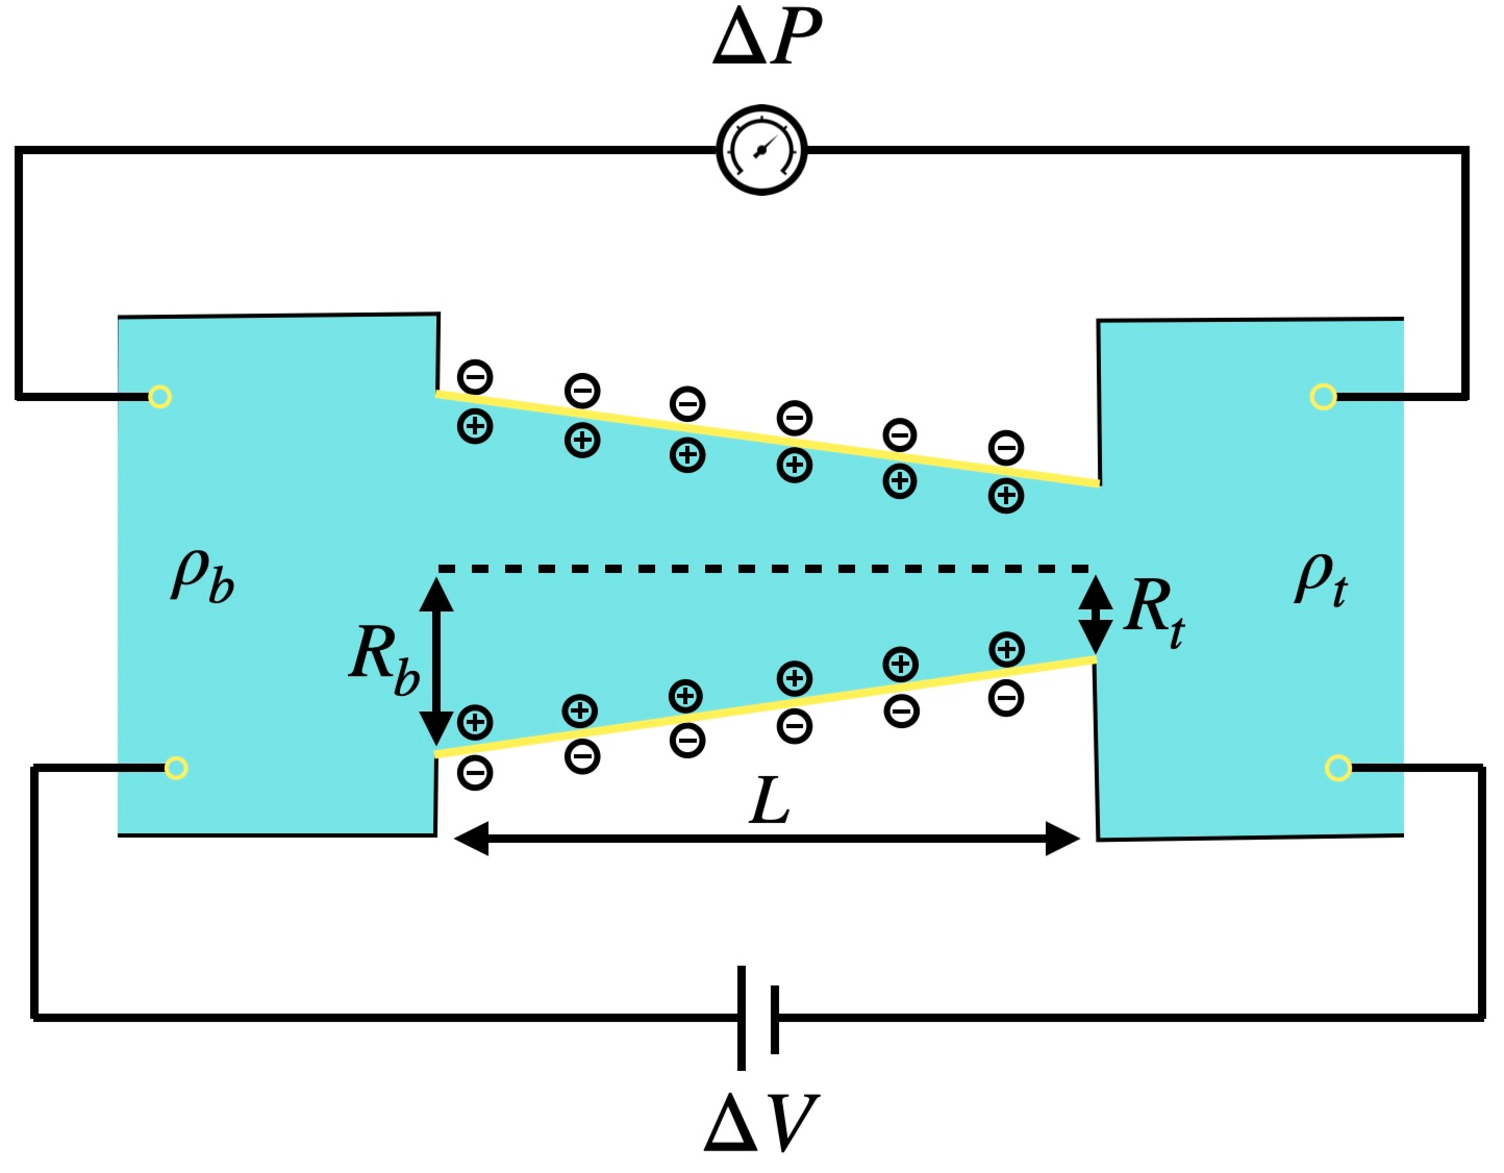
\includegraphics[width=\columnwidth]{plots/memristor/memristor_scheme.pdf}
    \caption{A schematic representation of the conical fluidic memristor. A cone of lenght $L$, base radius $R_b$ and tip radius $R_t$ with charged surface connnects two bulk reservoirs of a 1:1 electrolyte in an acqueous solution. The bulk density in the base $\rho_b$ differs from the bulk density in the tip $\rho_t$. At the far side of the memristor, an electrical potential and pressure drop are applied. Overall, this results in a chemical, electrical and mechanical sensistive system.}\label{fig:memristor_scheme}
\end{figure} 
An azimuthally symmetric conical channel connects two reservoirs that contain an incompressible aqueous 1:1 electrolyte with viscosity $\eta=1.01mPa s$ containing ions with diffusion coefficients $D = 1.75\mu m^2 ms^{-1}$ and charge $\pm e$ with $e$ the proton charge. The cone has a base radius of $R_b = 200$nm, a tip radius of $R_t=50$nm and has a length $L = 10\mu$m, which sets it in the long channel limit where entrance and exit effects can be neglected. The walls of the channel are homogeneously charged and generate a surface potential $\psi_0$ that attracts the opposite-sign ions present in the solution due to the dissociation of the electrolyte. The electric potential decreases exponentially away from the surface due to the electrostatic screening of the attracted ions: an electric double layer (EDL) forms on the charged surfaces. 

At the far side of both reservoirs, electrical potential, pressure and ion concentration are imposed. As a result, the memristor feels a potential drop $\Delta V = V_b - V_t$ defined as the difference between the potential in the base and in the tip. The ions within the EDL region generate an electro-osmotic fluid flow $Q_V = (\pi R_b R_t\epsilon\psi_0/L\eta)\Delta V$. Meanwhile, the pressure drop $\Delta P = P_b - P_t$, given by the difference between the base and the tip pressure, induces a Poiseuille-like flow $Q_P = (\pi R_b^3 R_t^3/8L\eta\langle R^2\rangle)\Delta P$. Finally, the ions experience a concentration gradient $\Delta \rho = \rho_b - \rho_t$, defined by the difference between the ion concentration in the reservoir connected to the base of the channel, $\rho_b$, and the concentration at the tip, $\rho_t$. Consequently, a diffusive fluid flow arises. However, we consider only the pressure and potential contributions to the total fluid flow, $Q = Q_P + Q_V$, assuming the diffusive flow to be negligible.  The resulting fluid flow generates non-trivial ion concentration profiles which, in turn, directly infulence the channel's conductance $g$. 
%It has already been shown that, for $\Delta P = 0$, the channel shows current rectification, thus working as a diode \cite{}, due to concentration polarization.  

In the steady-state, the channel is exposed to constant chemical, pressure and electrical signal, the corresponding conductance $g_{\infty}\brac{\boldsymbol{\Delta}}$ depends on the three stimuli $\boldsymbol{\Delta}= (\Delta V, \Delta P, \Delta \rho)$ and is determined by the ion concentration profiles according to 
\[
\frac{g_{\infty}\brac{\boldsymbol{\Delta}}}{g_0} = \int_0^{L} \frac{\bar{\rho}\left(x, \boldsymbol{\Delta}\right)}{2\rho_b L} dx                                           
\]
where $g_0$ is the Ohmic conductance and $\bar{\rho}(x)$ the radially averaged salt concentration as a function of $x\in[0,L]$\cite{Rene_IonicNeuromorphic}. By solving the stationary condition of the total salt flux, an expression for the average salt concentration can be found and reads
\begin{multline}
\frac{\bar{\rho}\left(x, \boldsymbol{\Delta}\right)}{2\rho_b} = 1 - \frac{\Delta \rho}{\rho_b} \mathcal{I}\left(x, \Delta V, \Delta P\right) \\
 + \frac{ \rho_{in}\left( \Delta V \right) }{2\rho_b \text{Pe}} \left[ \mathcal{F}(x) - \mathcal{I}\left(x, \Delta V, \Delta P\right) \right]
\label{eq:rho_average}
\end{multline}
where we defined, for the sake of simplicity and readability, two functions
\[
\mathcal{I}\left(x, \Delta V, \Delta P\right) = \frac{e^{\frac{x}{L}\frac{R_t^2}{R_b R(x)} \text{Pe}}-1}{e^{\frac{R_t}{R_b} \text{Pe}}-1}, \ \ \ \ \mathcal{F}(x) = \frac{x}{L}\frac{R_t}{R(x)}.
\]
Moreover, we introduced an expression for the concentration inhomogeneity 
\[
\rho_{in}\brac{\Delta V} = 2\frac{(R_b-R_t)\sigma}{R_t^2}\frac{e\Delta V}{k_B T}
\]
and the Péclet number
$
\text{Pe} = QL/D\pi R_t^2
$
which quantifies the importance of the flow $Q$ over diffusion \cite{Rene_PressureSensitive}.

%To better deal with numerical instabilities, we use a limit expression of \cref{eq:rho_average} when $\text{Pe} \ll \left( R_b/R_t \right)^2$ \cite{Rene_PressureSensitive}. With this consideration, the expression for the average salt concentration we use is the following
%\[
%\frac{\rho(x)}{2\rho_b} = 
%\begin{array}{cc}
 % \{ & 
  %  \begin{array}{cc}
   %   0 & x\leq 0 \\
    %  \frac{100-x}{100} & 0\leq x\leq 100
    %\end{array}
%\end{array}
%\]

When the external stimuli vary dynamically in time, they generate ion accumulation and deplition in the channel, changing consequently the conductivity. We assume the dynamics of the time-dependent conductance $g(t)$ as a single exponential decay towards the steady-state conductance $g_{\infty}$ with a diffusion-like timescale $\tau = L^2/12D$, as in Ref. \cite{Rene_IonicNeuromorphic}. The equation for the conductance reads
\begin{equation}
\frac{\partial g\brac{\boldsymbol{\Delta}(t), t}}{\partial t} = \frac{g_{\infty}\brac{\boldsymbol{\Delta}(t)}-g\brac{\boldsymbol{\Delta}(t), t}}{\tau}
\label{eq:eqofmotconductance}
\end{equation}
with $\boldsymbol{\Delta}(t) = \brac{\Delta V\brac{t},\Delta P\brac{t}, \Delta \rho\brac{t}}$.
As in Ref. \cite{Rene_IonicNeuromorphic}, we consider the time scale relative to voltage-driven ion accumulation or depletion in the channel. We justify this choice by stating that pressure-driven dynamics is faster and recalling that we neglect chemically-driven transport. Due to the fact that the conductance depends on the history of the signals applied, this system is called memristor. Aside from the direct dependence of the conductance on the external stimuli, there is an implicit dependence on the geometrical properties such as lenght $L$ and radius ratio $R_b/R_t$ that we choose to consider.

The PNN is composed of $\N$ nodes, an example is shown in \cref{fig:memristor_network}. 
\begin{figure}[h]
    \centering
    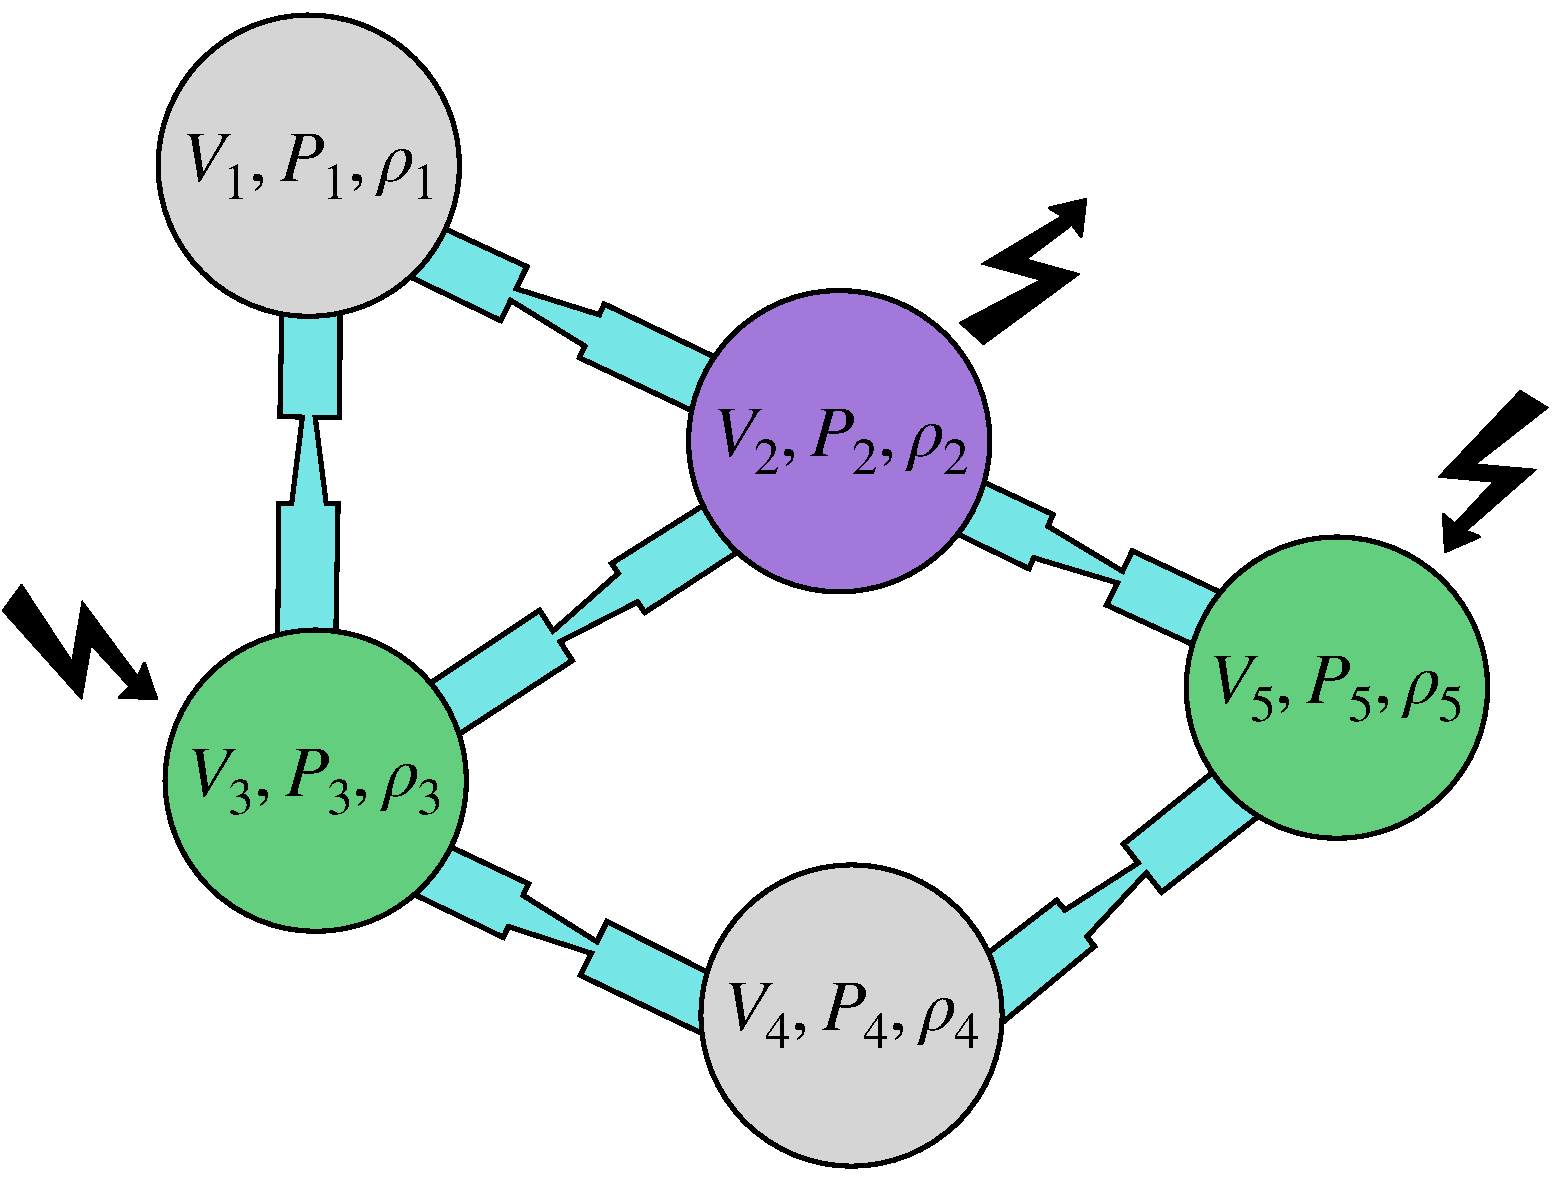
\includegraphics[width=0.8\columnwidth]{plots/memristor/memristor_network.pdf}
    \caption{An example of a network of five nodes connected by six memristors. The nodes are divided in input nodes (green circles), hidden nodes (gray nodes) and output nodes (purple circles) each of them is characterized by a triplet of physical quantities, representing the potential, pressure, and density. Th resulting stimuli on the memristor is given by the difference between base and tip signal, it thus depends on the oreintation of the memristor. In the case of the memristor that connects the first and the second node, for example, the exteranl stimuli are $\Delta V = V_2 - V_1$, $\Delta P = P_2 - P_1$ and $\Delta \rho = \rho_2 - \rho_1$. The zig-zag lines directed towards the input nodes indicate where the electrical signal is applied, while the zig-zag lines pointing outwards from the nodes indicate where the electrical signal is measured.}
    \label{fig:memristor_network}
\end{figure} 
Each node $\n\in[1,\N]$ is characterized by a value of electrical potential $V_{\n}$, pressure $P_{\n}$ and bulk density $\rho_{\n}$. Even though each node in the network is characterized by three physical properties, only electrical current flows through the network. This current propagates via the memristive elements, enabling modifications to the electric potential at other nodes. In contrast, pressure and density are externally imposed at each node and do not propagate through the network. The set of nodes is divided in thee sets. A node belongs to the set of \textit{input nodes} if it is used to imput current in the circuit, its value of voltage is known and fixed. After the imputs are imposed, the electrical signal travels throught the network and the resulting output potential is read in the nodes belonging to \textit{output nodes}. The remaining nodes, that do not function as input or output, are included in the set of \textit{hidden nodes}.

The nodes in the PNN are connected by $\M$ memristive elements. Consequently, a memristor connecting two nodes experinces potential drop, pressure drop and concentration gradient given by the difference between the node where the base of the memristor is connected to, and the node to which the tip is linked. The memristor is characterized by its conductance state $g_{\m}$ with $\m\in[1,\M]$, consequence of both the geomtery parameters and the external stimuli.

To solve numerically the resulting circuit, it is necessary to simultaneously address the circuit equations and the time evolution equation for the memristors' conductance. 
The circuit equations are handled using the open-source circuit solver \textsc{AHKAB}\cite{}, which computes the electric potentials at the nodes and the currents through the edges discretizing the differential equations in timesteps $\Delta t$. To incorporate the memristive elements, we approximate the time evolution of the conductances using a discretized form of \cref{eq:eqofmotconductance}, employing the Euler-forward method. Specifically, the conductance at a given timestep is calculated from its value at the previous timestep as:
\begin{multline}
g_{\m}\brac{\boldsymbol{\Delta}(t), t} = g_{\m}\brac{\boldsymbol{\Delta}(t), t-\Delta t} + \\
 \frac{g_{\m,\infty}\brac{\boldsymbol{\Delta}(t)-g_{\m}\brac{\boldsymbol{\Delta}, t}}}{\tau}\Delta t.
\end{multline}
In this work, we only apply constant voltage supplies to the input nodes of the circuit. Nonetheless, we notice that solving the dynamical equations is needed due to the dynamical change in the conductance of the memristors that, in turn, results in time-dependent potential drops across them.

\section{\label{sec:training}Training Algorithm for a Memristor Network}

As in a traditional algorithm for an ANN, the core mechanism of the training is to modify the weights associated to the connections of the network such that it maps specific inputs to desired outputs. In the case of the electrical network at hand, the training algorithm is designed to output desired voltage values in the output nodes, applying specific voltage values in the input nodes.
\begin{figure}[!h]
    \centering
    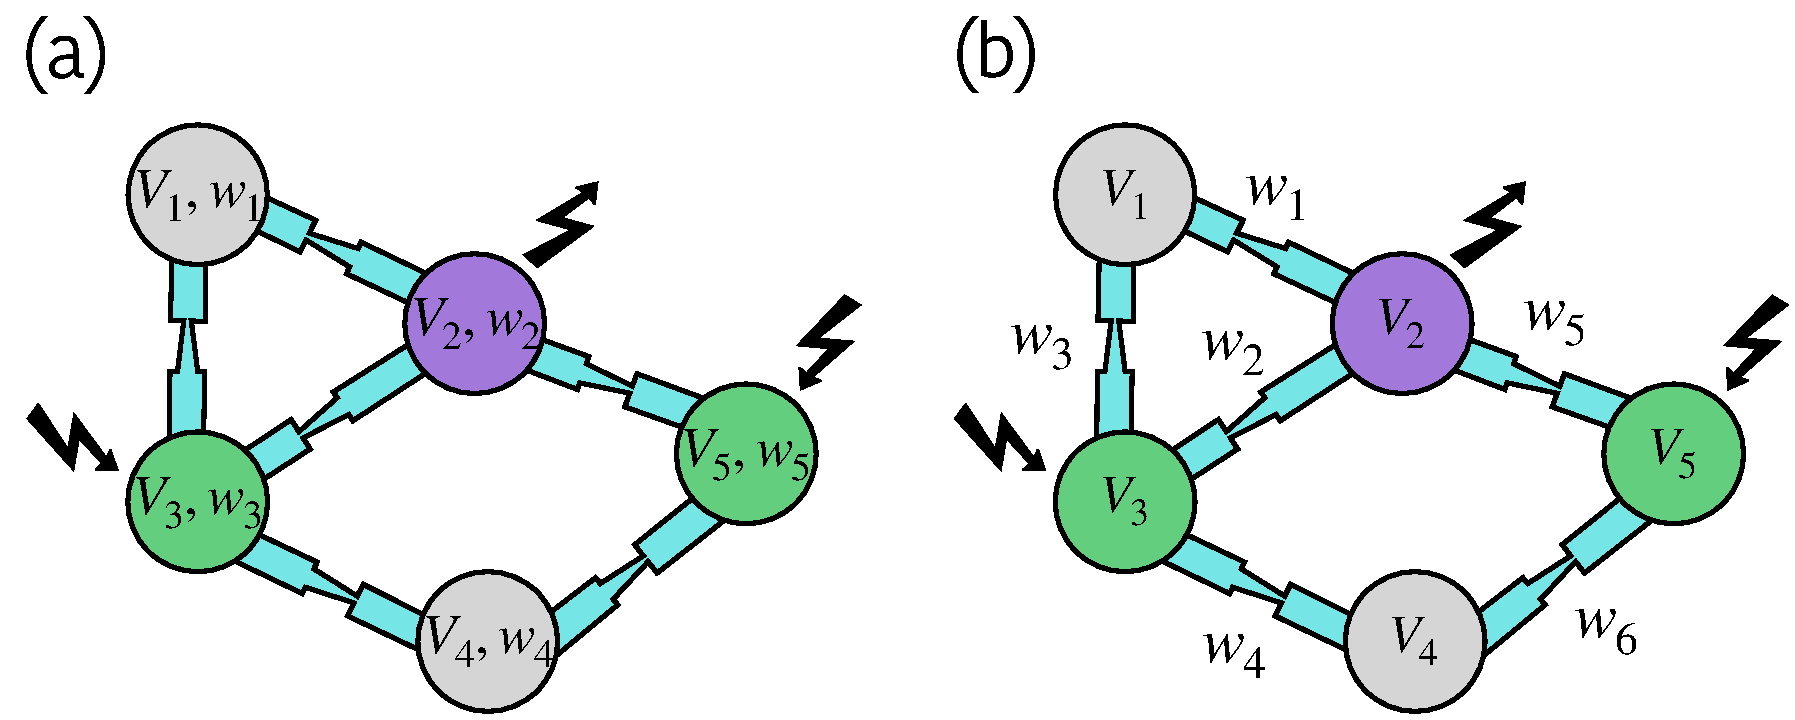
\includegraphics[width=0.8\columnwidth]{plots/training/two_types_weights.pdf}
    \caption{(a) Memristor network with weights defined in the nodes. (b) Memristor network where wegiths characterize each edge.}
    \label{fig:two_types_weights}
\end{figure} 
\begin{figure*}[t] 
    \centering
    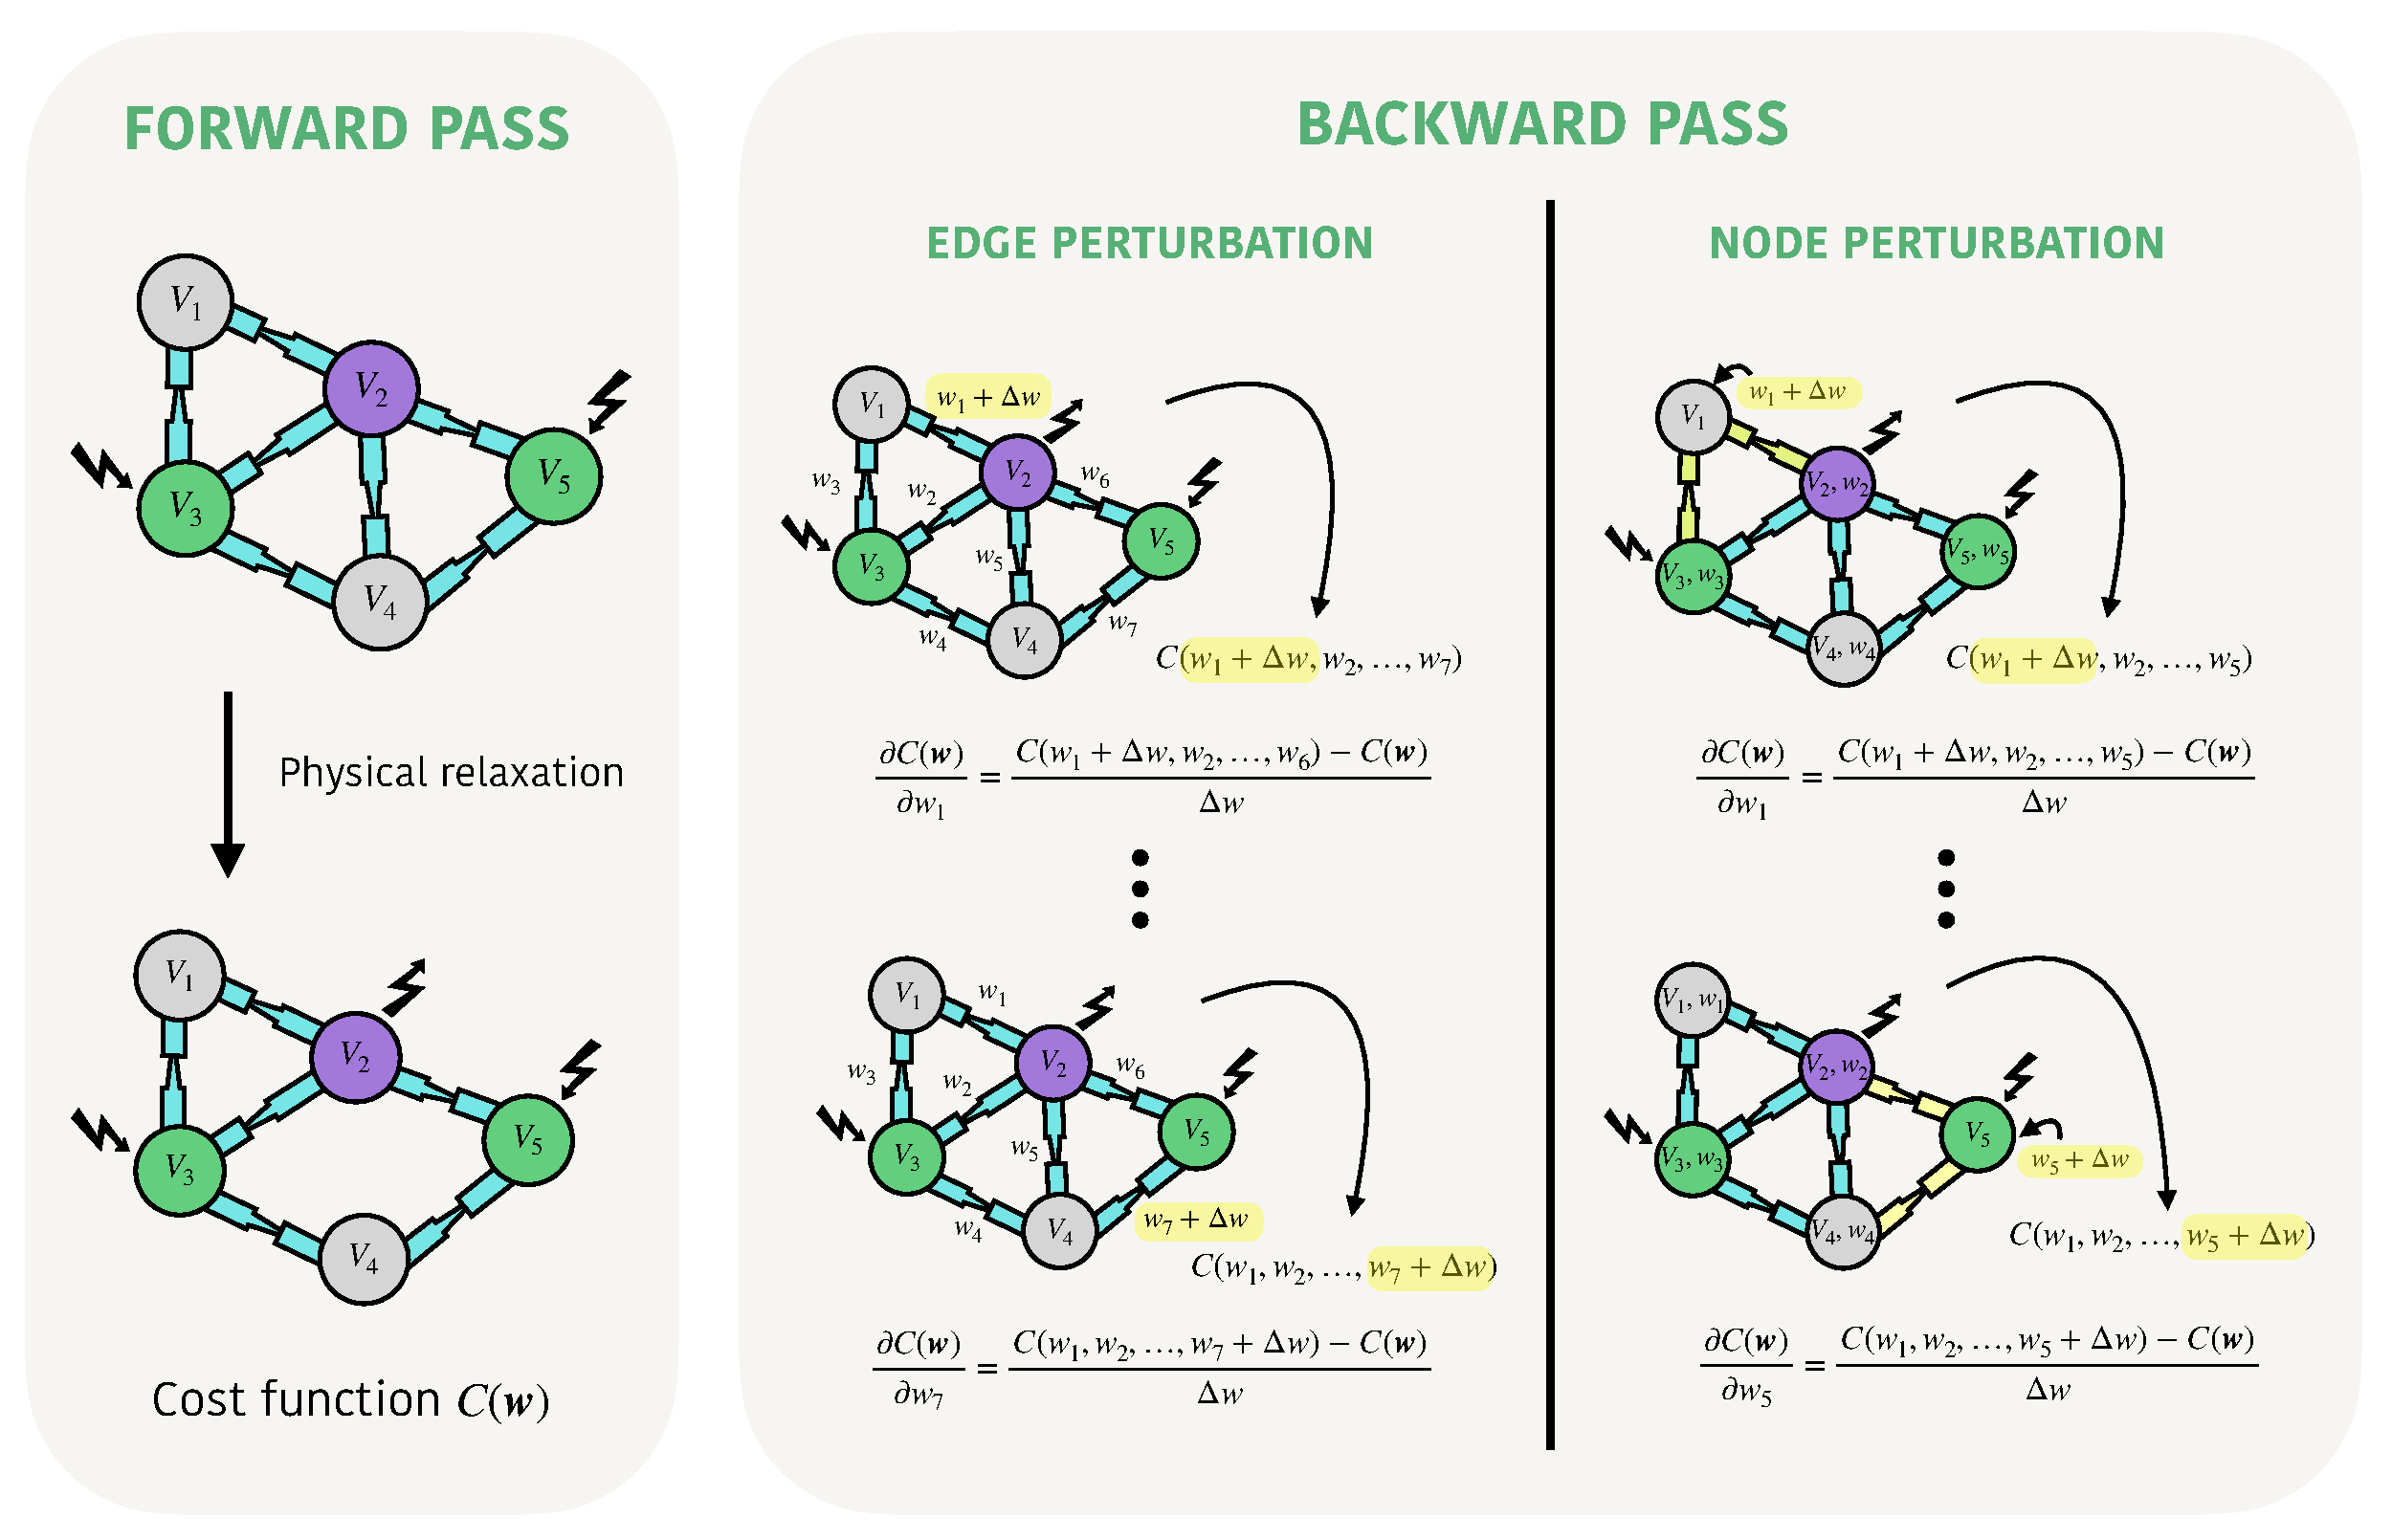
\includegraphics[width=\textwidth]{plots/training/training_scheme.pdf}
    \caption{}
    \label{fig:training_scheme}
\end{figure*}
Recalling that the dynamics of the memristors we consider depends on both external stimuli and geometrical properties, we have several possibilities for defining the weights of the network. However, there is a fundamental distinction between these two categories: external stimuli are applied to the nodes, while geometrical properties are defined edge-wise. Consequently, we distinguish between a training algorithm where the weights are defined on the nodes, as in \cref{fig:two_types_weights}(a), and one where the weights are defined on the edges, see \cref{fig:two_types_weights}(b). In this work, we focus on training a single property as the weight, while keeping all other parameters fixed as initially defined. For example, we may select an external stimulus, such as the imposed pressure or the density at each node. Alternatively, we can choose the length or radius ratio between the base and tip of the channel. The training process is carried out by iterating a scheme, illustrated in \cref{fig:training_scheme}, which consists of two phases: a forward pass and a backward pass.

In the feedforward phase, the network is fed with specific electric potential in the input nodes. Following both circuit laws and memristor's dynamics, the network reaches a steady state where electrical potentials can be measured in the output nodes. Clearly, the output of the network depends on the set of weights imposed on the network $\boldsymbol{w}$, regardless them being node or edge defined. The value of the outputs can be used to quantify the status of the network, meaning that it indicated how far the answer of the network is from the desired one. Specifically, we define a cost function that computes the difference squared between the voltage in the output nodes and the values of desired voltages
\[
C\left( \boldsymbol{w} \right) = \sum_{i \in \Lambda} \brac{V_i\brac{\boldsymbol{w}} - V_i^D}^2,
\]
where $\Lambda$ represents the set of indeces belonging to the output nodes, $V_i\brac{\boldsymbol{w}}$ the voltage measured in the output nodes and $V^D$ is a vector containing the values of desired output nodes.

The backward phase has the fundamental purpose of finding a set of weights that minimize the cost function. We follow the method of the \textit{steepest descent}, for which the update of the weights from one training step $s$ to the following $s+1$,
\begin{equation}
\boldsymbol{w}^{s+1} = \boldsymbol{w}^{s} - \alpha \boldsymbol{\nabla}C\brac{\boldsymbol{w}},
\label{eq:weight_update}
\end{equation}
results in a decrease in the cost funtion until a minimum is reached, for sufficienlty small values of $\alpha$ \cite{steepest_descent_book}. The gradient in the update rule is computed using a \textit{finite differences method}
\begin{equation}
\boldsymbol{\nabla}C\brac{\boldsymbol{w}} = \frac{C\brac{\boldsymbol{w}+\boldsymbol{\Delta w}}-C\brac{\boldsymbol{w}}}{\Delta w},
\label{eq:gradient_cost_func}
\end{equation}
where $\boldsymbol{\Delta w}$ is a vector with the same number of entries as the weight vector, but every entry has a value $\Delta w$. 

In the training algortihm, we first initialize the system with the memristor parameters specified in \cref{sec:memristor_network} and with some initial pressure and concentration values at each node. With the knowledge of input and desired output voltage values, it is possible to performe the first forward pass, from which we obtain the cost function $C\brac{\boldsymbol{w}}$, that we store since it is needed in the computation its gradient. Subsequently, we proceed with the backward pass. We compute each entry of the gradient in \cref{eq:gradient_cost_func} by selecting the corresponding weight, a node or an edge parameter, increment its value of $\Delta w$ and applying a forward step to obtain the corresponding entry of $C\brac{\boldsymbol{w}+\boldsymbol{\Delta w}}$. With the stored value of $C\brac{\boldsymbol{w}}$, we are able to compute the gradient in \cref{eq:gradient_cost_func} and use it to eventually calculate the weight update in \cref{eq:weight_update}.

Althought performed numerically in this work, we highlight that the feedforward pass is a physical process in which the system natually relaxes to its steady state. Moreover, also the backward pass we use can be translated to a physical event since involves performing the forward pass a number of time as the number of the weights. Once the cost functions are determined, only the simple algebric calculations of \cref{eq:weight_update} are left to be computed. We peopse this method as a hybrid physical and in-silico training algorithm also as a future experimental approach to the probelm.

\subsection{Training a Voltage Divider}

A voltage divider is an electrical circuit made of three nodes connected in series by two resistances, that returns a fraction of the input voltage. Given the simplicity of its structure, we use it as an initial playground for the training algorithm described above. Specifically, we replace the resistances with memristor channels, to be trained such that giving $V_1 = 5V$ and $V_3 = 0V$ as inputs, we get $V_2 = 4V$ as output. In \cref{fig:vd_scheme} a schematic of the memristor voltage divider is shown.

\begin{figure}[h]
    \centering
    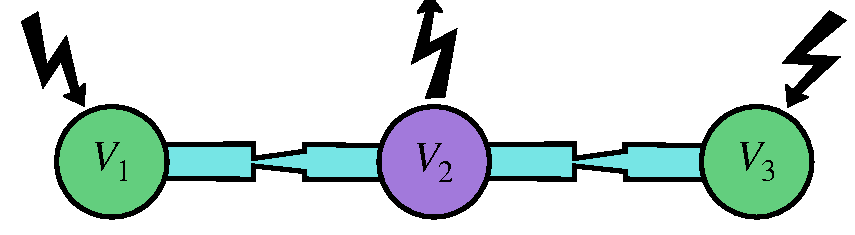
\includegraphics[width=0.8\columnwidth]{plots/voltage_divider/vd_scheme.pdf}
    \caption{}\label{fig:vd_scheme}
\end{figure} 

We initialize the system with pressures $P_1 =  P_2 = 1 bar$ and ion concetration $\rho_1 = \rho_2 = 0.2 mM$ on each node, length $L_1 = L_2 = 10\mu m$ and base radius  $R_{b1} = R_{b2} = 200 nm$ on each edge. After choosing one of these four physical quantities as training parameter $\boldsymbol{w} = \brac{w_1, w_2}$, we implement the training as descibed in \cref{sec:training} that modifies them, while the other parameters are kept constant. 
In \cref{fig:mse_weights_vd} we show that the cost function normalized to its initial value decreases of many order of magnitude during the training for each of the choosen weight. The values of the choosen set of weights simultaneouly changes from the initial condition, as shown in Figures [], adjusting the behaviour of the network to the desired one. In fact, if the values of a choosen type of weights at the end of the training are imposed to the netowork together with the voltage inputs, the network will autonomously realx to a staedy state that coincides with the desired state. To exemplify this point, the inset in Figure shows the physical relaxation of the voltage divider when the trained values of pressure, which correspond to the three values in the last training step, are imposed on the nodes together with the constant inputs voltages. The inset shows that the output voltage $V_2$ autonomously relaxes to the desired value of $V_D=3V$ in a time scale characteristic of the memristor.

\begin{figure}[h]
    \centering
    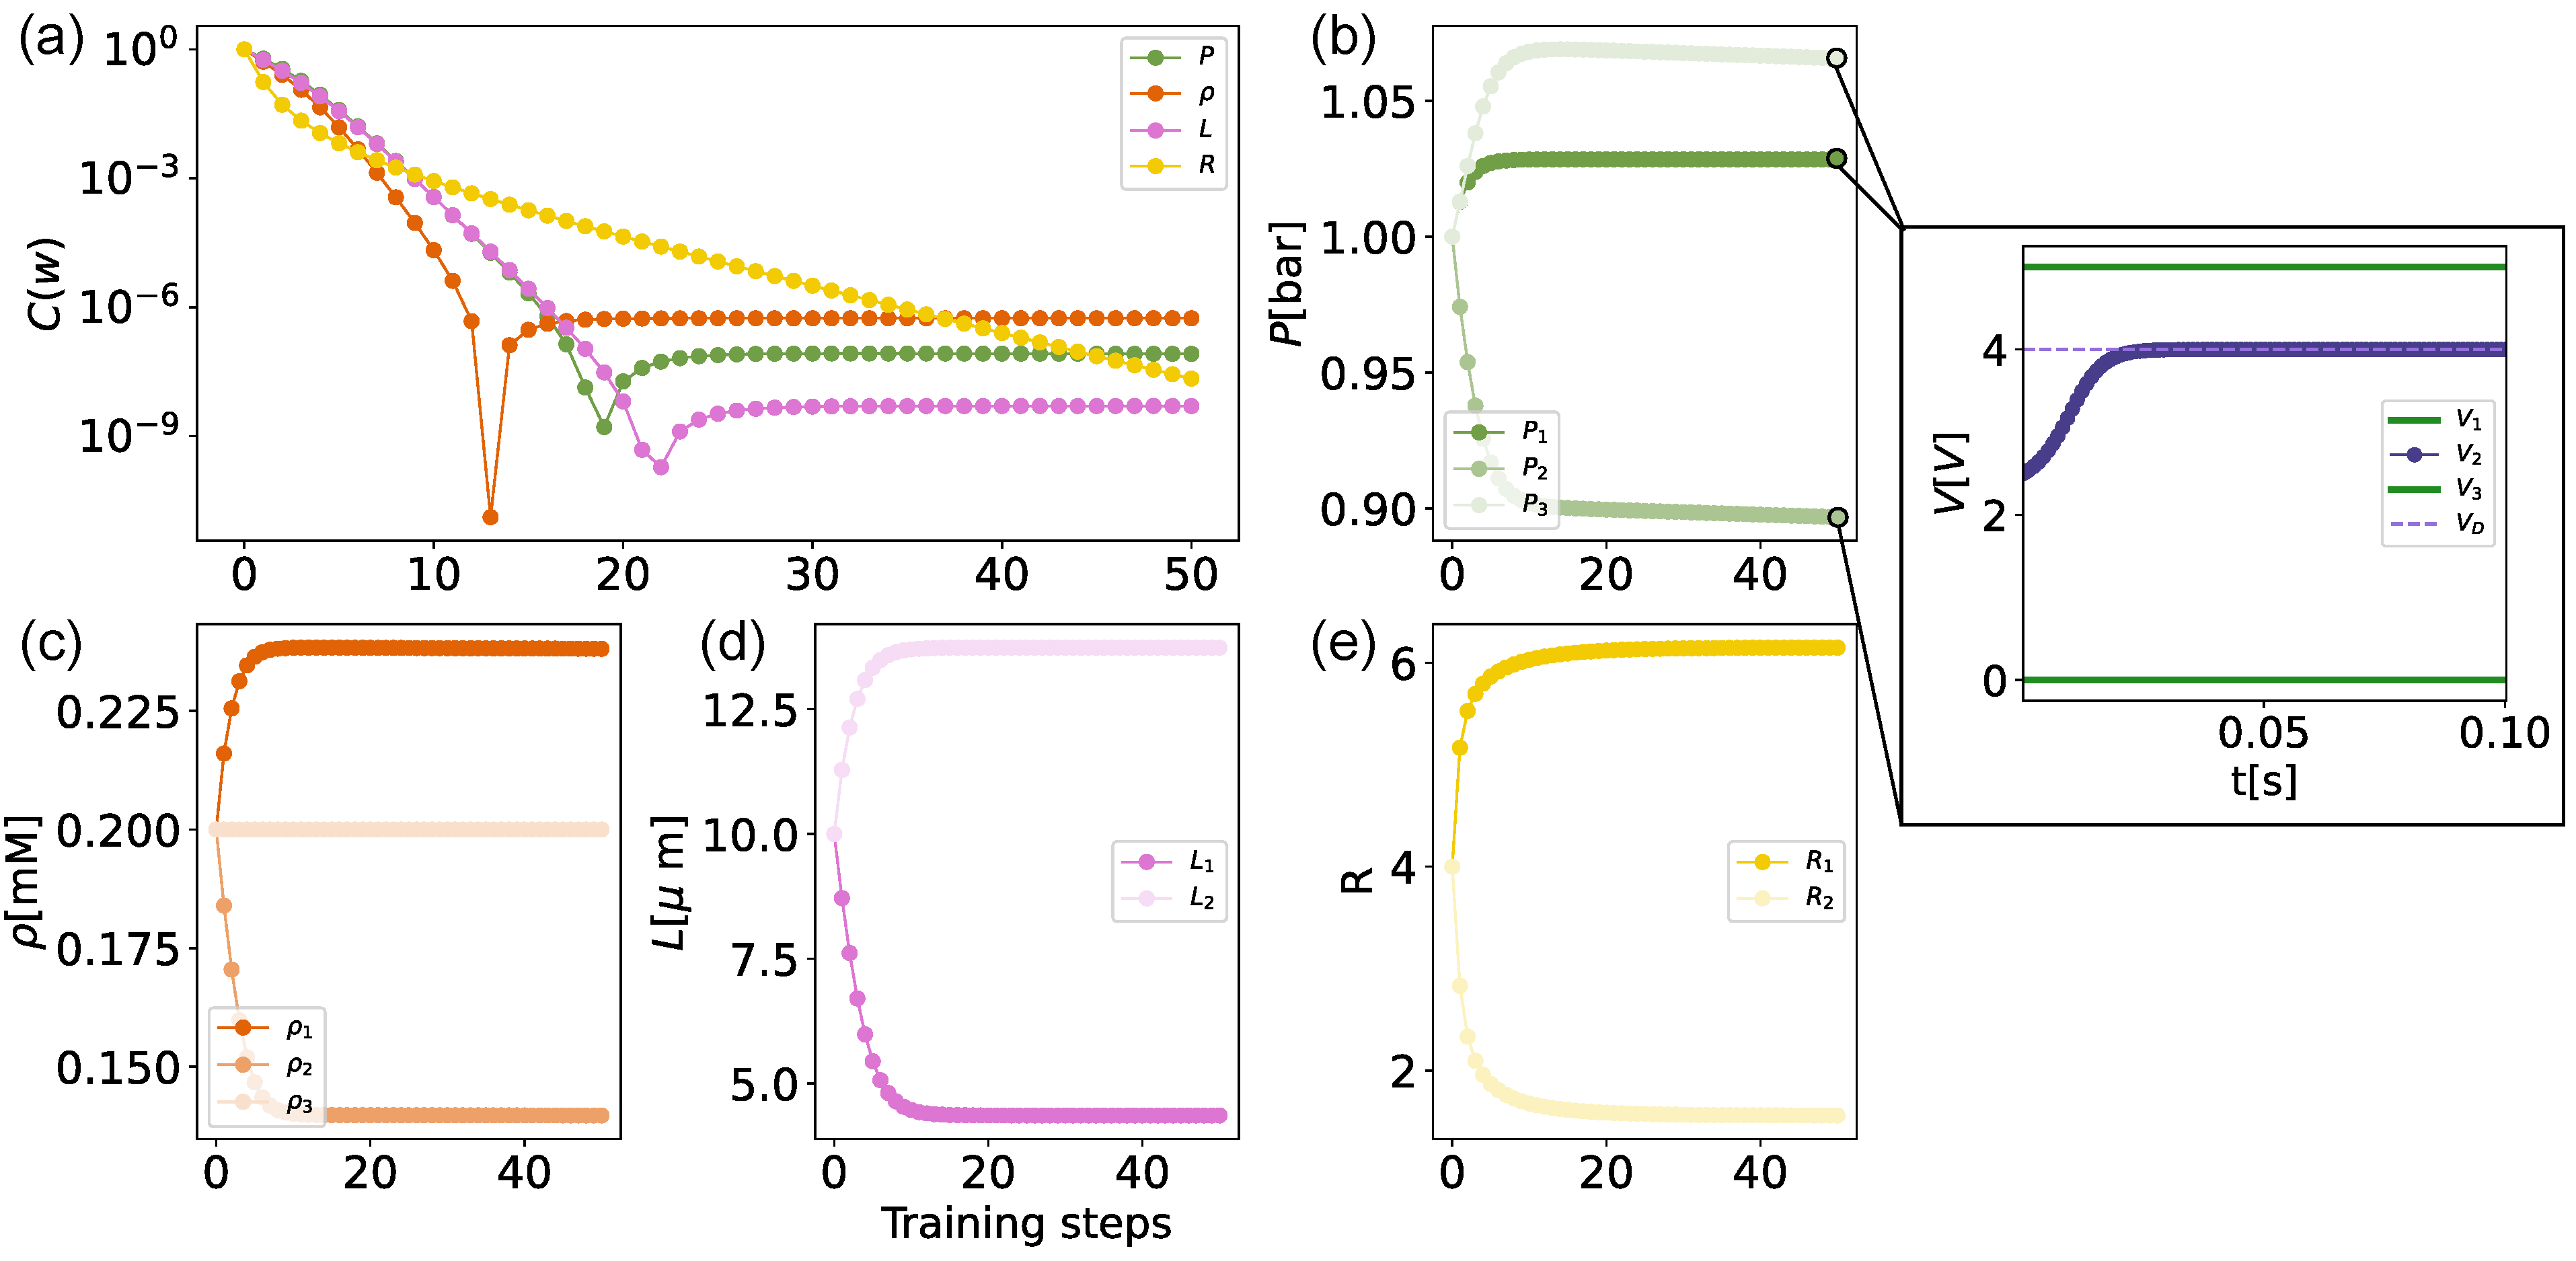
\includegraphics[width=\columnwidth]{plots/voltage_divider/mse_weights_vd.pdf}
    \caption{}\label{fig:mse_weights_vd}
\end{figure} 

\begin{figure}[h]
    \centering
    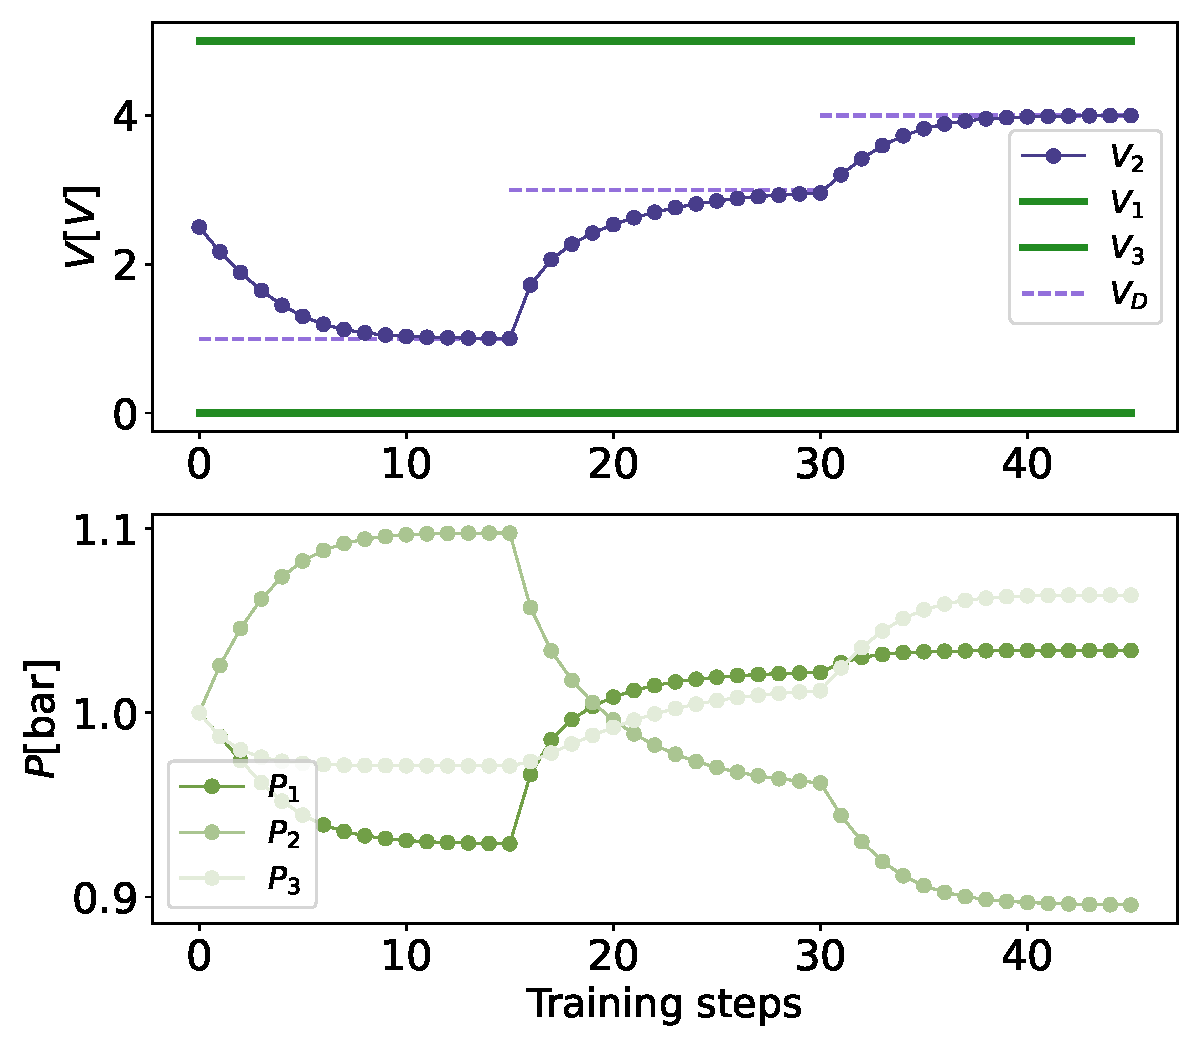
\includegraphics[width=0.8\columnwidth]{plots/voltage_divider/evolution_targets.pdf}
    \caption{}\label{fig:evolution_targets}
\end{figure} 

\cleardoublepage


\subsection{Training a more general network}

\begin{figure}[h]
    \centering
    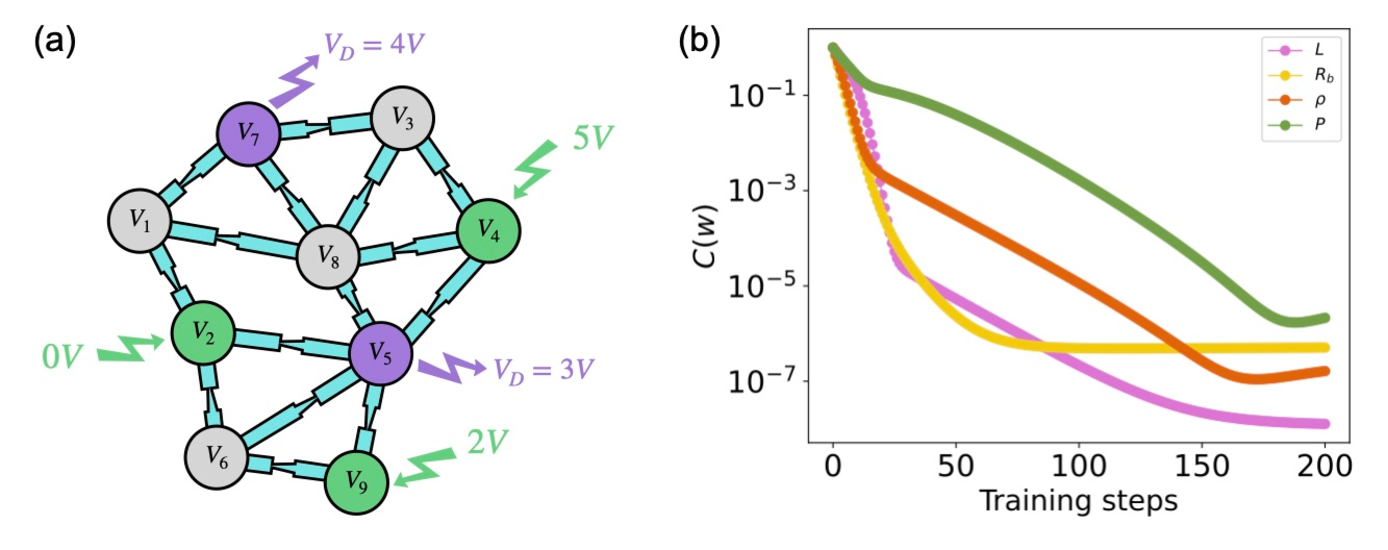
\includegraphics[width=\textwidth]{plots/general_network/mse_general.pdf}
    \caption{Network to the right has inputs $[5,0]$ nad desired outputs $[3, 4]$, delta weights a third of their intial value and learning rates $1e^{-5}, 1e^{-4}, 1e^{2}$. The network to the right has $[5,1,0]$ and output $[3,4,2]$}\label{fig:mse_general}
\end{figure} 



\cleardoublepage
\subsection{Linear Regression}

We broaden the training capability of the network by including a linear regression task, where, in its simplest form, the network is trained to give potential output $V^{\text{out}}$ related to the input potential $V^{\text{in}}$ via a linear relationship
\begin{equation}
    V_{\text{out}} = \text{c} V_{\text{in}} + \text{b}.
\label{eq:linear_relationship}
\end{equation}
% Firstly, we generate a data set of $$ input and output potential values, $\{ V^{in}_{i} \}_{i=1}^{}$ and $\{ V^{out}_{i} \}_{i}$ , that verify \cref{eq:linear_relationship}

\section{Conclusion}

\appendix




\clearpage
\bibliographystyle{unsrt} 
\bibliography{biblio}

\end{document}
